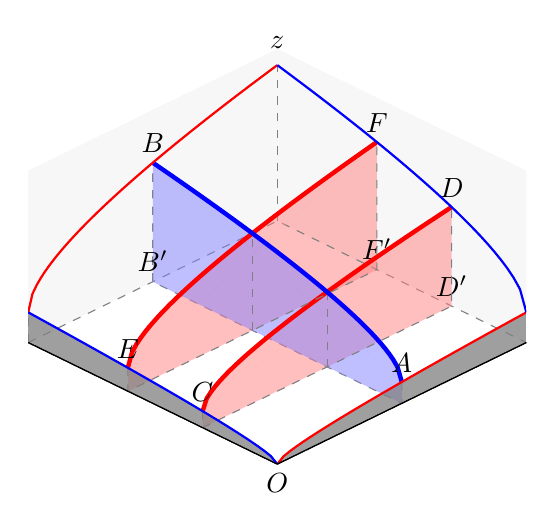
\begin{tikzpicture}
%(x^0.5 + 1) (y^0.5 + 1) - 1
\begin{axis}[
domain=0:10,
axis on top=true,
view={-45}{45},%view={-25}{60},
xmin=0,xmax=10,ymin=0,ymax=10,zmin=0,zmax=18,
xtick=\empty,ytick=\empty,ztick=\empty,
xticklabel=\ ,yticklabel=\ ,zticklabel=\ ,
width=180pt,height=150pt,
scale only axis,
axis x line*=middle,
axis y line*=middle,
axis z line*=none,
axis line style={-},
extra x ticks={5,9},
extra x tick style={tickwidth=0},
extra x tick labels={$A'$,$x$},
extra y ticks={3,6,9},
extra y tick style={tickwidth=0},
extra y tick labels={$C'$,$E'$,$y$},
extra description/.code={
	\node[below] at (axis cs:0,0,0) {$O$};
	\node[above] at (axis cs:10,10,17) {$z$};
},
axis background/.style={fill=black!3}]
\addplot3[fill=white,draw=none] coordinates {
(0,0,0)
(0,10,0)
(10,10,0)
(10,0,0)
};

\addplot3[gray,dashed,thin] coordinates {
(5,0,2.236)
(5,0,0)
(5,10,0)
(5,10,12.469)
};

\addplot3[fill=red!50,draw=none,fill opacity=0.5] coordinates {
(0,6,0)
(0,6,2.449)
(10,6,13.358)
(10,6,0)
};

%----------------------------------------------------------------------
\addplot3[gray,dashed,thin] coordinates {
(0,10,0)
(10,10,0)
(10,0,0)
};
%补偿z轴
\addplot3[gray,dashed,thin] coordinates {
(10,10,0)
(10,10,16.324)
};
%补偿xymax的纵向边界
\addplot3[gray,dashed,thin] coordinates {
(0,10,0)
(0,10,3.163)
};
\addplot3[gray,dashed,thin] coordinates {
(10,0,0)
(10,0,3.163)
};
%----------------------------------------------------------------------
%y=3 z=z(x) 观察x的边际效用递减
%只是填充
\addplot3[draw=none,samples=60,samples y=0,fill=red!50,fill opacity=0.5] ({x},{3},{sqrt(3)+(1+sqrt(3))*sqrt(x)}) --cycle;
%拼凑
\addplot3[fill=red!50,draw=none,fill opacity=0.5] coordinates {
(0,3,0)
(0,3,1.732)
(10,3,10.372)
(10,3,0)
};
\node[above] at (axis cs:10,3,0) {$D'$};
%----------------------------------------------------------------------
%y=6 z=z(x) 观察x的边际效用递减
%只是填充
\addplot3[draw=none,samples=60,samples y=0,fill=red!50,fill opacity=0.5] ({x},{6},{sqrt(6)+(1+sqrt(6))*sqrt(x)}) --cycle;
%拼凑
%\addplot3[fill=red!50,draw=none,fill opacity=0.5] coordinates {
%(0,6,0)
%(0,6,2.449)
%(10,6,13.358)
%(10,6,0)
%};
\node[above] at (axis cs:10,6,0) {$F'$};
%----------------------------------------------------------------------
%x=5 z=z(y) 观察y的边际效用递减
%只是填充
\addplot3[draw=none,samples=60,fill=blue!50,fill opacity=0.5] ({5},{y},{sqrt(5)+(1+sqrt(5))*sqrt(y)}) --cycle;
%拼凑
\addplot3[fill=blue!50,draw=none,fill opacity=0.5] coordinates {
(5,0,2.236)
(5,0,0)
(5,10,0)
(5,10,12.469)
};
\node[above] at (axis cs:5,10,0) {$B'$};
%----------------------------------------------------------------------
%绘制上述截面的交线
\addplot3[gray,dashed,thin] coordinates {
(5,3,0)
(5,3,7.841)
};
\addplot3[gray,dashed,thin] coordinates {
(5,6,0)
(5,6,10.163)
};
%----------------------------------------------------------------------
%y=3 z=z(x) 观察x的边际效用递减
\addplot3[draw=red,ultra thick,samples=60,samples y=0] ({x},{3},{sqrt(3)+(1+sqrt(3))*sqrt(x)});
\addplot3[gray,dashed,thin] coordinates {
(0,3,1.732)
(0,3,0)
(10,3,0)
(10,3,10.372)
};
\node[above] at (axis cs:0,3,1.732) {$C$};
\node[above] at (axis cs:10,3,10.372) {$D$};
%----------------------------------------------------------------------
%y=6 z=z(x) 观察x的边际效用递减
%主要曲线
\addplot3[draw=red,ultra thick,samples=60,samples y=0] ({x},{6},{sqrt(6)+(1+sqrt(6))*sqrt(x)});
%辅助线
\addplot3[gray,dashed,thin] coordinates {
(0,6,2.449)
(0,6,0)
(10,6,0)
(10,6,13.358)
};

\node[above]  at (axis cs:0,6,2.449) {$E$};
\node[above] at (axis cs:10,6,13.358) {$F$};
%----------------------------------------------------------------------
%x=5 z=z(y) 观察y的边际效用递减
\addplot3[draw=blue,ultra thick,samples=60] ({5},{y},{sqrt(5)+(1+sqrt(5))*sqrt(y)});
%\addplot3[gray,dashed,thin] coordinates {
%(5,0,2.236)
%(5,0,0)
%(5,10,0)
%(5,10,12.469)
%};
\node[above] at (axis cs:5,0,2.236) {$A$};
\node[above]  at (axis cs:5,10,12.469) {$B$};
%----------------------------------------------------------------------
\addplot3[draw=none,fill=gray,fill opacity=0.75,samples=40,samples y=0] ({x},{0},{sqrt(x)}) \closedcycle ; 
\addplot3[draw=none,fill=gray,fill opacity=0.75,samples=40] ({0},{y},{sqrt(y)}) \closedcycle;
%----------------------------------------------------------------------
%绘制曲面与坐标系边界的交线
%(x^0.5 + 1) (y^0.5 + 1) - 1
\addplot3[draw=red,thick,samples=40,samples y=0] ({x},{0},{sqrt(x)}); %samples=100,samples y=0
\addplot3[draw=red,thick,samples=60,samples y=0] ({x},{10},{4.16*(sqrt(x)+1)-1});
\addplot3[draw=blue,thick,samples=40] ({0},{y},{sqrt(y)});
\addplot3[draw=blue,thick,samples=40] ({10},{y},{4.16*(sqrt(y)+1)-1});
\end{axis}
\end{tikzpicture}